\documentclass[10pt,twocolumn,letterpaper]{article}

\usepackage{iccv}
\usepackage{times}
\usepackage{epsfig}
\usepackage{graphicx}
\usepackage{amsmath}
\usepackage{amssymb}
\usepackage{indentfirst}
\usepackage{subcaption}

% Include other packages here, before hyperref.

% If you comment hyperref and then uncomment it, you should delete
% egpaper.aux before re-running latex.  (Or just hit 'q' on the first latex
% run, let it finish, and you should be clear).
\usepackage[breaklinks=true,bookmarks=false]{hyperref}
\setkeys{Gin}{width=\columnwidth}
\graphicspath{{pictures/}}
\iccvfinalcopy % *** Uncomment this line for the final submission

\def\iccvPaperID{****} % *** Enter the ICCV Paper ID here
\def\httilde{\mbox{\tt\raisebox{-.5ex}{\symbol{126}}}}

% Pages are numbered in submission mode, and unnumbered in camera-ready
%\ificcvfinal\pagestyle{empty}\fi
\setcounter{page}{1}
\begin{document}

%%%%%%%%% TITLE
\title{A Review Of Immersive Scientific Visualization}

\author{Zhongyuan Yu\\
{\tt\small algoyu@163.com}
% For a paper whose authors are all at the same institution,
% omit the following lines up until the closing ``}''.
% Additional authors and addresses can be added with ``\and'',
% just like the second author.
% To save space, use either the email address or home page, not both
\and
Stefanie Krell\\
{\tt\small stefanie.krell@mailbox.tu-dresden.de}
}

\maketitle
%\thispagestyle{empty}


%%%%%%%%% BODY TEXT
\section{Introduction}
%The use of stereoscopic images can improve the depth cue and the perception of the spatial relationships which might be crucial for scientist when analyzing data.
Scientific Visualization is the visualization of scientific phenomena. The purpose is to enable scientists to understand, illustrate and get insight from their data. The data arising from observations or simulations has an implicit or explicit geometric structure, is often very large and most of the time in 3D. Phenomena that can be visualized include the visualization of particles, terrain, volume, flow and tensors.

\setlength{\parindent}{1pc}Virtual reality (VR) can give a sense of presence or immersion in 3D environments. It is a class of computer-controlled multisensory communication technologies that allow more intuitive interactions with data and involve human senses in new ways. An illusion of a three-dimensional world is generated with a stereoscopic head-tracked display system. Nowadays head mounted displays (HMDs) like Oculus Rift1 or HTC Vive2 are widely available and therefore also used in scientific visualization. There are also VR systems like the CAVE (released in 1992) \cite{cruz1992cave}: an immersive virtual reality environment where projectors are directed to the walls of a room-sized cube. It uses a motion capture system, which records the real time position of the user for interaction. VR-systems provide many of the depth cues which we use in the real world, such as binocular disparity and head-motion-parallax. The perception of spatial relationships is highly improved in comparison to 2D displays. When using VR for Scientific visualization, scientists can explore the data in ways which might lead to insights they would otherwise not get because of the increased depth perception and improved interaction with the studied object/phenomena. 

\setlength{\parindent}{1pc}Earliest publications about VR in scientific visualization can be found in the 1990s. Steve Bryson \cite{bryson1994virtual} discussed the use of VR in Scientific Visualization in 1994. He basically concluded that virtual environments provide significant advantages for complex three-dimensional phenomena but drawbacks were high cost of hardware. As technologies evolved costs decrease and display resolutions are higher, VR technologies provide better immersion into a virtual worlds than back in the 90s. Since there has been done a lot of research on this topic in the past decades, we will focus on four new projects from the last 6 years, which are more relevant for today's research. Those projects are using different forms of visualizations: particle visualization, point-cloud visualization and volume visualization. Three of them are using HMDs and one is for the CAVE2 \cite{febretti2013cave2}. We will discuss the rendering techniques and interaction techniques each approach is using. One thing all four approaches have in common is the fact that they have to deal with high amount of data and therefore apply different optimization strategies.

\setlength{\parindent}{1pc}The paper can be divided into 6 chapters. In the second chapter we will present challenges proposed in a approach of point cloud visualization \cite{discher_point-based_2018}. In the following chapter we will discuss a project, which is about tracing neurons in microscopy data \cite{} by. Chapter 4 will discuss a ray-tracing approach for molecular visualization \cite{}. Chapter 5 will describe the techniques used for the visualization of atomistic simulations \cite{reda_visualizing_2013}. The last part will conclude the topic, point out remaining challenges and state some future work.

\section{Point Cloud Visualization}
\subsection{Overview}
Discher et al. \cite{discher_point-based_2018} utilized a multi-pass rendering pipeline to visualize 3D point clouds with different rendering techniques on VR Head Mounted Displays. 3D point clouds are data sets which come from 3D scans e.g. via Airborne (Fig. \ref{fig:pointcloud_1}), Terrestrial or Mobile Laser scanning. They are used in areas like geospatial and non-geospatial applications, building information modeling, urban planning and cultural heritage. Real time rendering of 3D points clouds allows for interactive exploring of real-world assets, sites or regions. As this field has to deal with high amount of data the main challenge is to balance between render quality and performance. In VR on HMDs, the applications have to cope with additional problems: stereoscopic rendering, very high frame rates (90fps as opposed to 30-60fps to avoid nausea, the feeling of motion sickness) and high sensitivity to any kind of visual artifacts which are typical for showing 3D Point Clouds (e.g holey surfaces and visual clutter). The project allows for exploration of 3D point clouds with VR devices such as HTC Vive or Oculus Rift. The algorithm was tested with up to 2.6 billion points. The goal of this project was to show the scalability and practicability of the approach. 

This project is similar to the approaches that are explained in section 3 and 4 as it is designed for visualization on HMDs rather than an immersive environment like introduced in the approach in section 5. Discher et al. \cite{discher_point-based_2018} took a lot of emphasis on the analyzing the visual quality rather than mostly the run time. The visualized data set differs a lot from all the other data sets, because points rather than particles or volumes are visualized.
\begin{figure}
	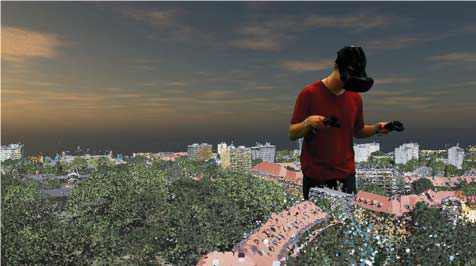
\includegraphics{pointcloud_1.png}
	\caption{Point-cloud Visualization on HTC Vive of an Airborne scan of a city}
	\label{fig:pointcloud_1}
\end{figure}
\subsection{Rendering}
\begin{figure}
		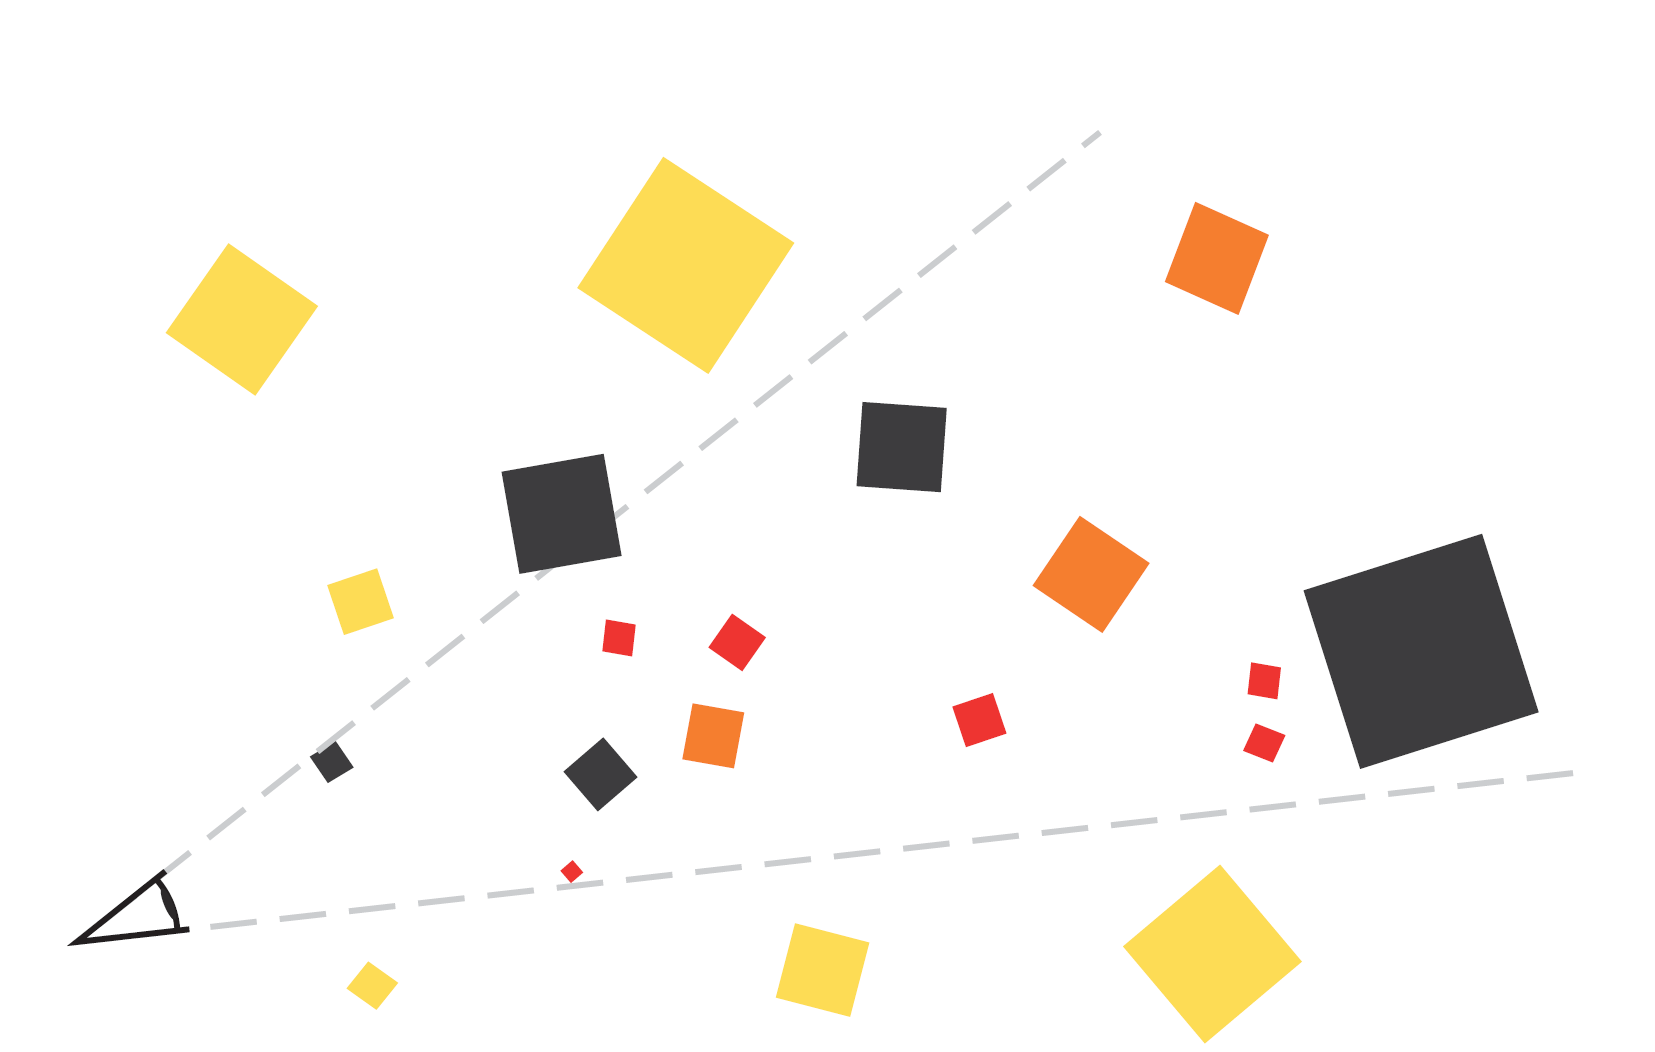
\includegraphics{pointcloud_2.png}
	\caption{Culling techniques used to reduce the amount
of points to be rendered: View frustum culling (yellow),
occlusion culling (orange), detail culling (red).}
	\label{fig:pointcloud_2}
\end{figure}
\begin{figure}
		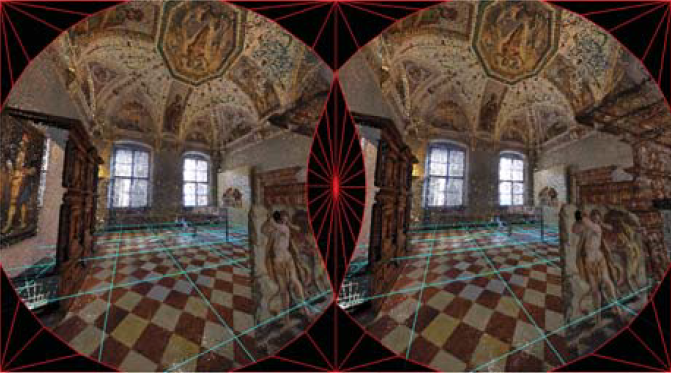
\includegraphics{pointcloud_3.png}
	\caption{A separately rendered mesh serves as a mask to discard fragments beyond the visible area of an VR device’s screens early on}
	\label{fig:pointcloud_3}
\end{figure}
A variety of optimization techniques for rendering were implemented to cope with the performance and visual problems arise when rendering massive 3D point clouds especially on VR devices. Former approaches had to reduce the precision and density of the data by thinning the point clouds \cite{kreylos2008immersive} or converting them into generalized 3D meshes \cite{berger2017survey}. The rendering system of the introduced approach consists of three basic steps: data subset selection, point cloud rendering and image-based post processing.

\setlength{\parindent}{1pc}Data subset selection is necessary because presentation and interactive visualization of 3D point clouds have to deal with the massive amount of data, which generally exceeds available CPU and GPU capabilities. For this reason out-of-core rendering concepts and spatial data structures are required. The 3D point cloud is subdivided in a representative subset that fit into GPU and CPU storage, which can be used for real-time rendering. Here, they determined the subset on a per-frame basis. Firstly, points outside the view frustum are excluded (Fig. \ref{fig:pointcloud_2}). The second technique they used, is detail culling (Fig. \ref{fig:pointcloud_2}). Very small details contribute little. If the estimated area of an object is below a certain pixel threshold, the object is discarded. As an explicit Level-of-Detail (LoD) structure to provide efficient access to the data they are using kd-trees. It is a binary tree whose splitting planes can be chosen on the respective coordinate axes. This allows for minimal traversal times during rendering and the tree structure is balanced independent of the spatial position of points. Other acceleration data structures which have been used for point cloud rendering are quadtrees \cite{Gao:2014:VAL:2619648.2619672} or octrees \cite{kreylos2008immersive}. Schuetz et al. \cite{schuetz-2019-CLOD} proposed a different approach for rendering point clouds in VR. They utilized a continuous LoD structure instead of an explicit one. A flat array is used as a data structure with the hierarchy level stored in an attribute. It exhibits gradual rather than sudden changes in density. The issue which comes due to chunked LoD representation is addressed. It avoids hierarchical traversal, as no tree structure is used. The change of detail is less noticeable. But this approach is limited to point-clouds that fit in GPU memory.

\setlength{\parindent}{1pc}The next step Discher et al. \cite{discher_point-based_2018} called point cloud rendering. The data subset is rendered into g-buffers. That are specialized frame buffer objects (FBO) that combine multiple 2D textures (color, depth, normal). During run time, it is possible to select different rendering techniques and change the appearance of the point cloud. They implemented three different rendering techniques trying to improve the performance. First one is the Hidden mesh rendering (Fig. \ref{fig:pointcloud_3}). The actual visible area on screen on VR devices is restricted to a circular area. To prevent a lot of unnecessary fragment shader operations, a mesh representing the hidden parts of the screen as a mask is used to discard those fragments early on \cite{vlachos_advanced_2015} with early fragment testing. That is possible by using the depth or stencil buffer, which is executed before the fragment shader when using early fragment testing. Next implemented technique is the reverse painters algorithm \cite{foley1996computer}, which is a GPU-based occlusion culling technique based on early fragment testing. Occluded fragments  are not processed by the fragment shader. Scene objects should be rendered in order of their distance to the view position for the technique to have a measurable effect. That is done on a per node basis of the kd-tree rather than per point bases to increase performance. Both of these techniques improved the performance but it varies depending on the number of fragments. The third rendering technique is single-pass stereo rendering, which has the goal to reduce the CPU-overhead by rendering both views of right and left eye in a single render pass \cite{johansson2016efficient}. The frame buffer size is doubled, as each half is assigned to one eye. Instanced rendering, which is a way to render multiple instances of a object in a single draw call and provide each instance with some unique attributes, is used to prevent duplicated draw calls. This technique proved to be less effective because the main performance bottleneck was the GPU rather than the CPU. 

\setlength{\parindent}{1pc}In addition to those, Discher et al. \cite{discher_point-based_2018} implemented two rendering techniques that are supposed to improve the image quality. That is necessary as the impressiveness of a scene is negatively effected by any kind of visual artifact. The most noticeable artifacts due to inappropriately sized points are the holey appearance of surfaces or visual clutter. One technique that was used is the adaptive point size, which works on a per node basis of the kd-tree. For each node they determine its deepest descendant that has been selected for rendering. To all its ancestors the adaptive point size is applied. The point sizes are calculated based on a node’s bounding box rather than its LoD, since nodes of the same LoD might still have quite different point densities. But the visual artifacts are not completely removed. Another rendering technique which was applied is paraboloid rendering \cite{schutz2016potree}. It aims to reduce the visual clutter further by rendering points as paraboloids oriented towards the viewing direction rather than screen aligned disks. A depth offset is added to fragments, which depends on the distance to the corresponding point's center. Undesired occlusions are reduced significantly. But it is not compatible with the rendering techniques using early fragment testing, because the depth is modified in the fragment shader. This technique should only be used carefully as it decreases the performance significantly.

\setlength{\parindent}{1pc}The final step of the used rendering pipeline is imaged-based post processing. It operates on previously generated g-buffers. The post processing should improve the image quality further. Those techniques are screen space ambient occlusion (SSAO) (efficiently approximates the ambient occlusion effect in real-time) \cite{mittring2007finding} and eye-dome lighting (EDL) \cite{boucheny2009interactive}, which add depth cues and highlight silhouettes, blurring \cite{lukin2016tips}, which smooths aliasing and z-fighting (two or more primitives have similar or identical values in the z-buffer). Furthermore, remaining holes are filled and two one-dimensional filter kernels \cite{dobrev2010image} instead of a single two dimensional one for a performance speed up, are applied. The authors of the paper suggested to not use every image improvement techniques as they would slow down the rendering a lot.

\subsection{Interaction}
The VR environment is not only used for displaying. Controllers are used for interaction to improve the experience and exploration. Rotating and scaling of the rendered data is supported, as well as measuring distance between points, and selection of applied rendering technique and color.
\subsection{Conclusion}
The multi-pass approach offers a maximum degree of freedom as rendering techniques can be adjusted at run time. It is highly beneficial for applications in digital documentation, preservation, and presentation of natural and cultural heritage, because it allows user to remotely explore. Future work can focus on performance improvements by distributing the stereo rendering across two separate GPUs.

\section{Tracing Neurons}
\subsection{Overview}
To understand the coordinated activity of neurons in brain has become a central goal of neuroscience nowadays. That means we have to know the location of billions of interconnected neurons and understand the connections between them. Obviously, it takes huge amount of time and a lot of effort without a computer-aided system. For most of the 20th century, reconstructing, annotating, and analyzing neurons has been done by creating hand-drawn images of labeled neurons, traced using an instrument known as camera lucida directly from thin brain sections viewed through a microscope\cite{Usher2018}. Even some newly developed systems for tracing neurons are reported to have drawbacks like NeuroLucida(the current industry standard for neuron tracing) \cite{lucida2018} and TeraFly plugin for Vaa3D \cite{v3d}. Besides, some automatic techniques for neuron reconstruction will fail on complex and noisy data. Peng et al.\cite{Peng2011} has reported that the clean-up process may take longer than manual tracing. Current systems should be improved with more advanced methods.

\begin{figure}[h]
\begin{center}
%\fbox{\rule{0pt}{2in} \rule{0.9\linewidth}{0pt}}
   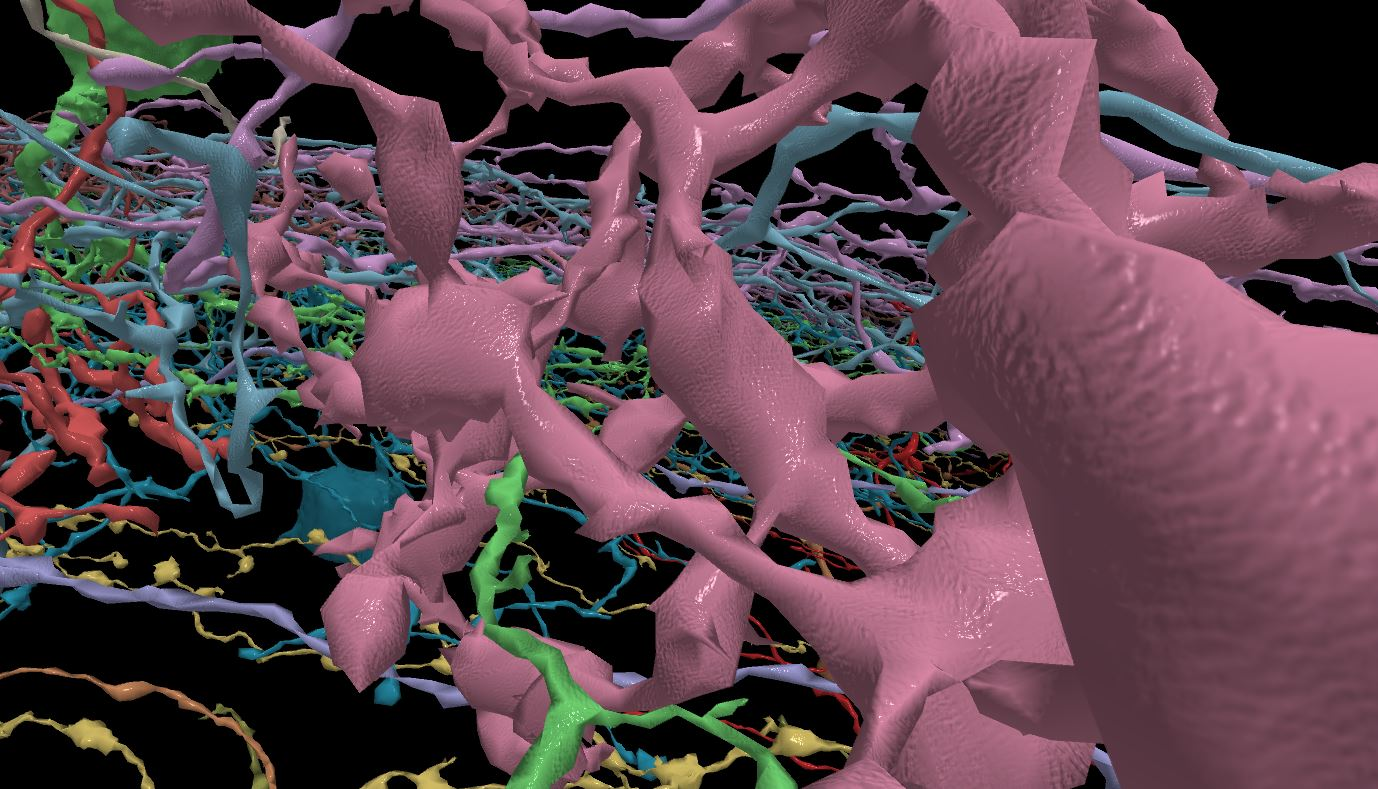
\includegraphics[width=1.0\linewidth]{gen.png}
\end{center}
   \caption{Rendering neuron connection with mesh. The colors for each neuron in the mesh vertices has been encoded.A technique called tri-planar texture mapping has been used to add a normal map without using UV coordinates, giving the models a shiny/bumpy look up close.}
\label{fig:gen}
\end{figure}

Usher et al.\cite{Usher2018} has reported a novel approach to trace neuronal circuits in brain. It is a interdisciplinary research which provides a solution for connectomics researchers with virtual reality technology. The main goal of this project is to improve the quality and speed of neuron tracing, which is achieved by different innovative rendering, interaction, and navigation methods. There are some similar projects like The Virtual Finger in Vaa3D and NeuroLucida 360. These methods provides semi-automatic extraction approaches which improves the speed at which neuron morphology can be traced. But they are viewpoint and visibility dependent. Which means that they can be very slow when the data size increases. Also, Jeong et al \cite{Jeong2010} combine segmentation and stitching analysis with an out-of-core GPU volume renderer for large datasets.
\subsection{Rendering}
Difficulties in rendering neuron with HMDs are found in state-of-art methods. It presents a significant challenge to avoid motion sickness with both high-resolution and frame-rate requirements. Low frame rates and pauses during computation are not as tolerable as the case in traditional desktop visualization. With HMDs, we have a limited time to render each frame, which is only about 11ms. Compared to our VRAM of current GPUs(4-24GB) and RAM(64-128GB) space in our computers nowadays, the neuron datasets can be very large, range from hundreds of gigabytes to terabytes \cite{Usher2018}. Thus, we need to work with data stream. It is reported in this project that only 2ms is budgeted for data streaming on the render thread, which is very short. Moreover, it is common to step inside the dataset. When walking through the volume, it is observed that the scene begin to vibrate, this should be eliminated for a better experience. After that, We need to correctly composite the geometry, wands, and tracings when using volume rendering technique. At the same time, Depth perception can be challenging in volume rendering, when we just use gradient shading. Thus, it might hard to determine the exact position of the wands in this case. Furthermore, when enhancing the depth perception with isosurface rendering mode, the result can not be ideal due to the noisy data.

The author of paper \cite{Usher2018} has presented novel approaches to solve the problems above. To avoid motion sickness they take cues from VR game development \cite{Vlachos2015}. They have designed a streamlining rendering pipeline, in which they submit draw calls approximately equal to 2ms before VSync. At the same time, the asynchronous volume data will be uploaded based upon the user’s focus region instead of the whole scene. It is a strictly budgeting work which improves the rendering performance significantly. To deal with huge amount of data with a limited rendering time, they provided a data streaming solution. At the same time, they use a two-level caching system in it: the first level loads and caches pages from disk into RAM, and the second level takes these pages and uploads them to the GPU \cite{Baker:1977} . A faster data loading process can be achieved by reducing disk access frequency and latency to display pages with the caching system above. On an other hand, they presents a scheme to restrict the visible popping of pages. That is, they load a box slightly larger than the focus region and prioritize pages closer to the user’s view(Fig. \ref{fig:neuron-render}). This scheme of limiting the enqueueing rate has been found simpler than updating priorities for already scheduled pages. To avoid vibrate effect when wandering across the datasets, they begin sampling at the sample point nearest to the clipping plane this is similar to \cite{291532}. To do composition with the geometry, wands, and tracings correctly, in the ray marching step, they use the depth buffer produced by rendering the opaque geometry to terminate rays early. Moreover, Shadows or global illumination which are advanced rendering techniques that can improve the perception of depth. But those techniques are computational expensive, and hard to apply in a VR setting if we want to maintain a sufficient frame rate for VR. The author of this paper does not use those techniques due to their significant frame-rate or memory cost. Instead, they added the ability to switch to an implicit isosurface mode, with Phong shading and ambient occlusion. To deal with noisy data in the implicit isosurface mode, they de-noise the data first. More precisely, they filter out objects less than 11 voxels in size before uploading the page to the GPU by finding small connected components.

\begin{figure}[h]
\begin{center}
%\fbox{\rule{0pt}{2in} \rule{0.9\linewidth}{0pt}}
   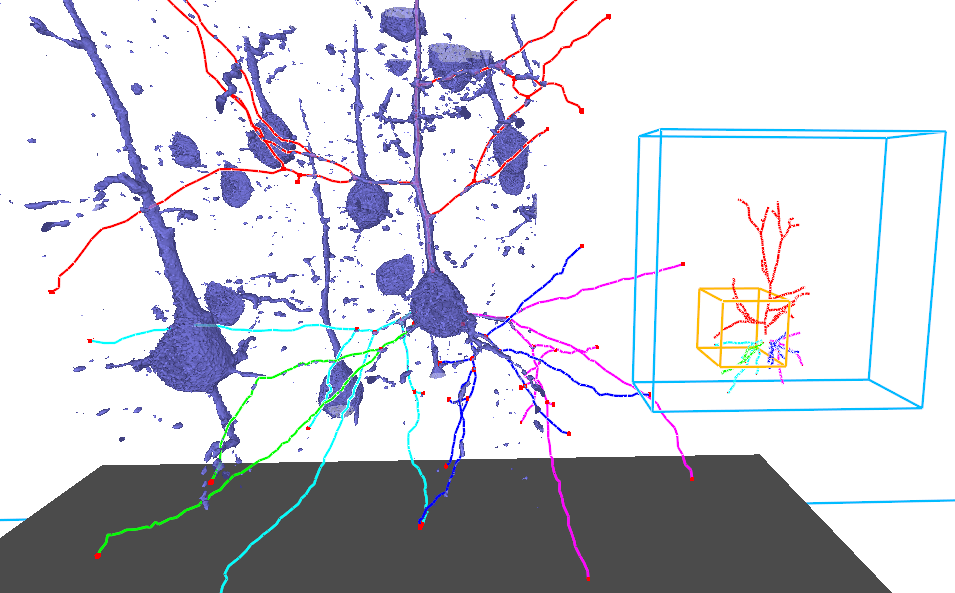
\includegraphics[width=1.0\linewidth]{neuron-render.png}
\end{center}
   \caption{A screenshot of the system, using the isosurface rendering mode. With the help of minimap (right), Users can orient themselves in the dataset. It shows the world extent in blue, the current
focus region in orange, and the previously traced neuronal structures.}
\label{fig:neuron-render}
\end{figure}

\subsection{Interaction}
Tracing and navigation are key tasks when reconstructing neurons. Difficulties can be found in state-of-art methods to achieve this. There is a problem when designing the interaction model: what to use and how to use interaction tools. If we have designed something that hard to navigate through the dataset, it will be less powerful when used by experts from the field of neuron research. Besides, We have to make sure that the correctness of tracing the branches of a neuron can easily be achieved. That means, the tracing of branches must be easy (Fig. \ref{fig:neurou-tracing}). Additionally, It is always a good idea to give feedback to the user during the interaction in a system. Thus, we have to call attention to the user when they are trying to select something.

\begin{figure}[h]
\begin{center}
%\fbox{\rule{0pt}{2in} \rule{0.9\linewidth}{0pt}}
   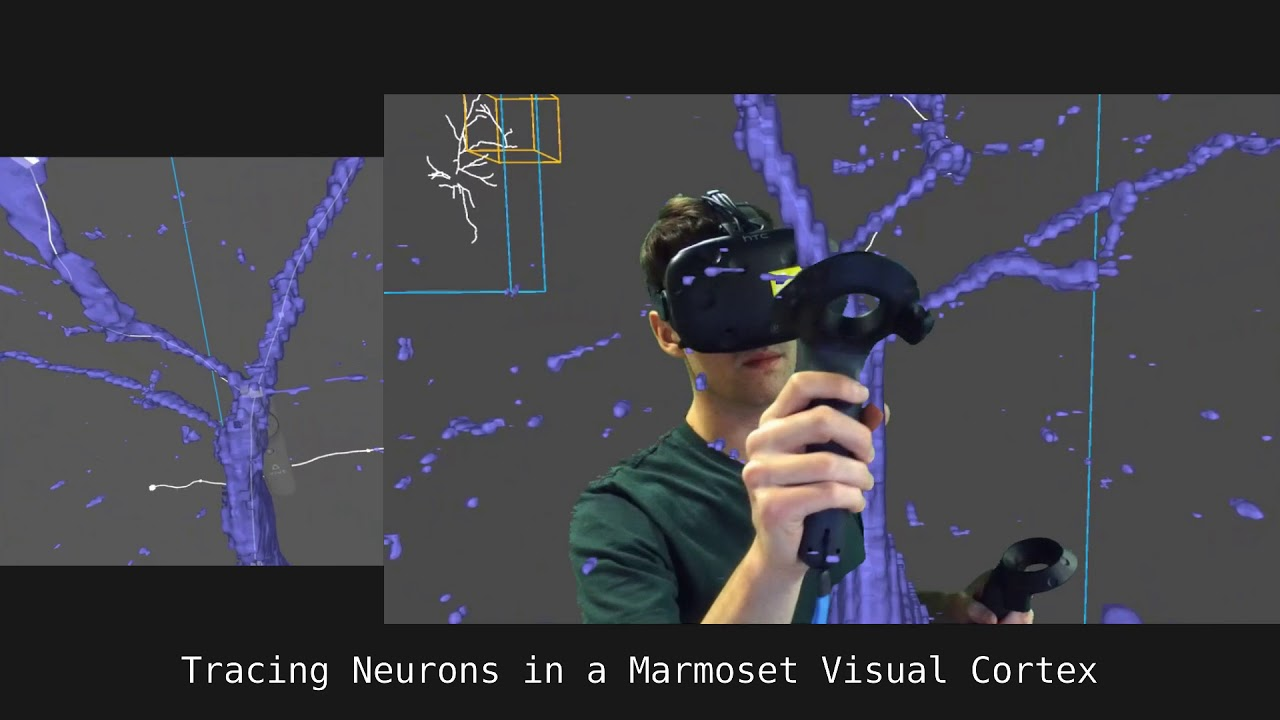
\includegraphics[width=1.0\linewidth]{neurou-tracing.png}
\end{center}
   \caption{Navigating through large-scale dataset using VR controller: navigation wand. That handheld controller also enables us throwing, steering and aiming in VR scene.}
\label{fig:neurou-tracing}
\end{figure}

\begin{figure}[h]
\begin{center}
%\fbox{\rule{0pt}{2in} \rule{0.9\linewidth}{0pt}}
   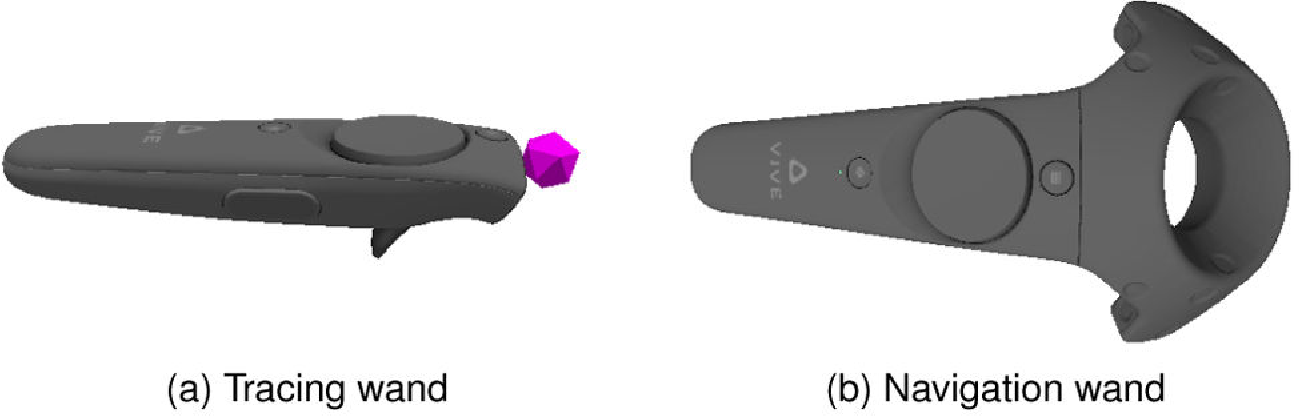
\includegraphics[width=1.0\linewidth]{wands.png}
\end{center}
   \caption{The button sticking out underneath (a) is
the trigger, and the large circular button is the trackpad. The icosphere
brush in (a) is colored to match the selected line color.}
\label{fig:wands}
\end{figure}

In this project \cite{Usher2018} , they use the wand model with two wands: One is used for tracing and the other for navigation (Fig. \ref{fig:wands}). The actions are initiated by holding the trigger button on the corresponding wand to avoid spurious triggering. The navigation wand is rendered to match the wand’s physical model to avoid motion sickness. The user then holds the trigger she or she follows the neuron through the data, drawing a line from the brush. Releasing the trigger ends the line and creates the termination point. The user is then free to continue the line from the termination point, or trace branches as needed \cite{Usher2018}. This is the key interaction process designed in that paper. It makes users easier to navigate large dataset, which motivates users to work in a immersive way and have a better understanding of it at the same time. The creation of a branch in their system is easy, by letting users to select different drawing methods instead of just one. The user can start a new line along the current tracing and follow the neuron branch out, or start a new line on the neuron branch and reconnect to the parent tree. To call attention to the reconnection, they highlight the selected node and send a small vibrationto the wand to give a “click” feeling of selecting it. Also, they display a small cube to indicate where the branching point will be placed. The visual and physical feedback provides a clear signal to the user that the desired operation has been done. By importing those feedback methods, the interaction between the user and the system is enhanced.
\section{Molecular Visualization}
\subsection{Overview}
Molecular visualization in virtual reality can be useful for visualizing and analyzing molecular structures and three-dimensional (3D) microscopy by providing intuitive perception of complex structures \cite{Xu589366}. Virtual reality (VR) offers immersive display with a wide field of view and head tracking for better perception of molecular architectures and uses 6-degree-of-freedom hand controllers for simple manipulation of 3D data \cite{6DOF}. Which helps scientists to gain a better understanding of their data. The increase in the knowledge of macromolecular structures lets scientists to understand the real world better. Software packages for this purpose can easily be found. Such as VMD \cite{VMD}, a well-known molecular visualization program for displaying, animating and analyzing large biomolecular systems using 3D graphics and built-in scripting. PyMOL \cite{pymol}, a Python-enhanced molecular graphics tool that normally runs on desktop machines. But most of them only work on a desktop PC. Nowadays consumer VR headsets are affordable to researchers and educators. Thus, pushing the scientific visualization applications to virtual reality environment becomes a research topic. However, due to the need for low-latency, high-frame-rate rendering, it is challengeable to be realized in HMDs without so-called simulator sickness \cite{LaViola:2000}. At the same time, new interaction problems should also be solved.

\begin{figure}[h]
\begin{center}
%\fbox{\rule{0pt}{2in} \rule{0.9\linewidth}{0pt}}
   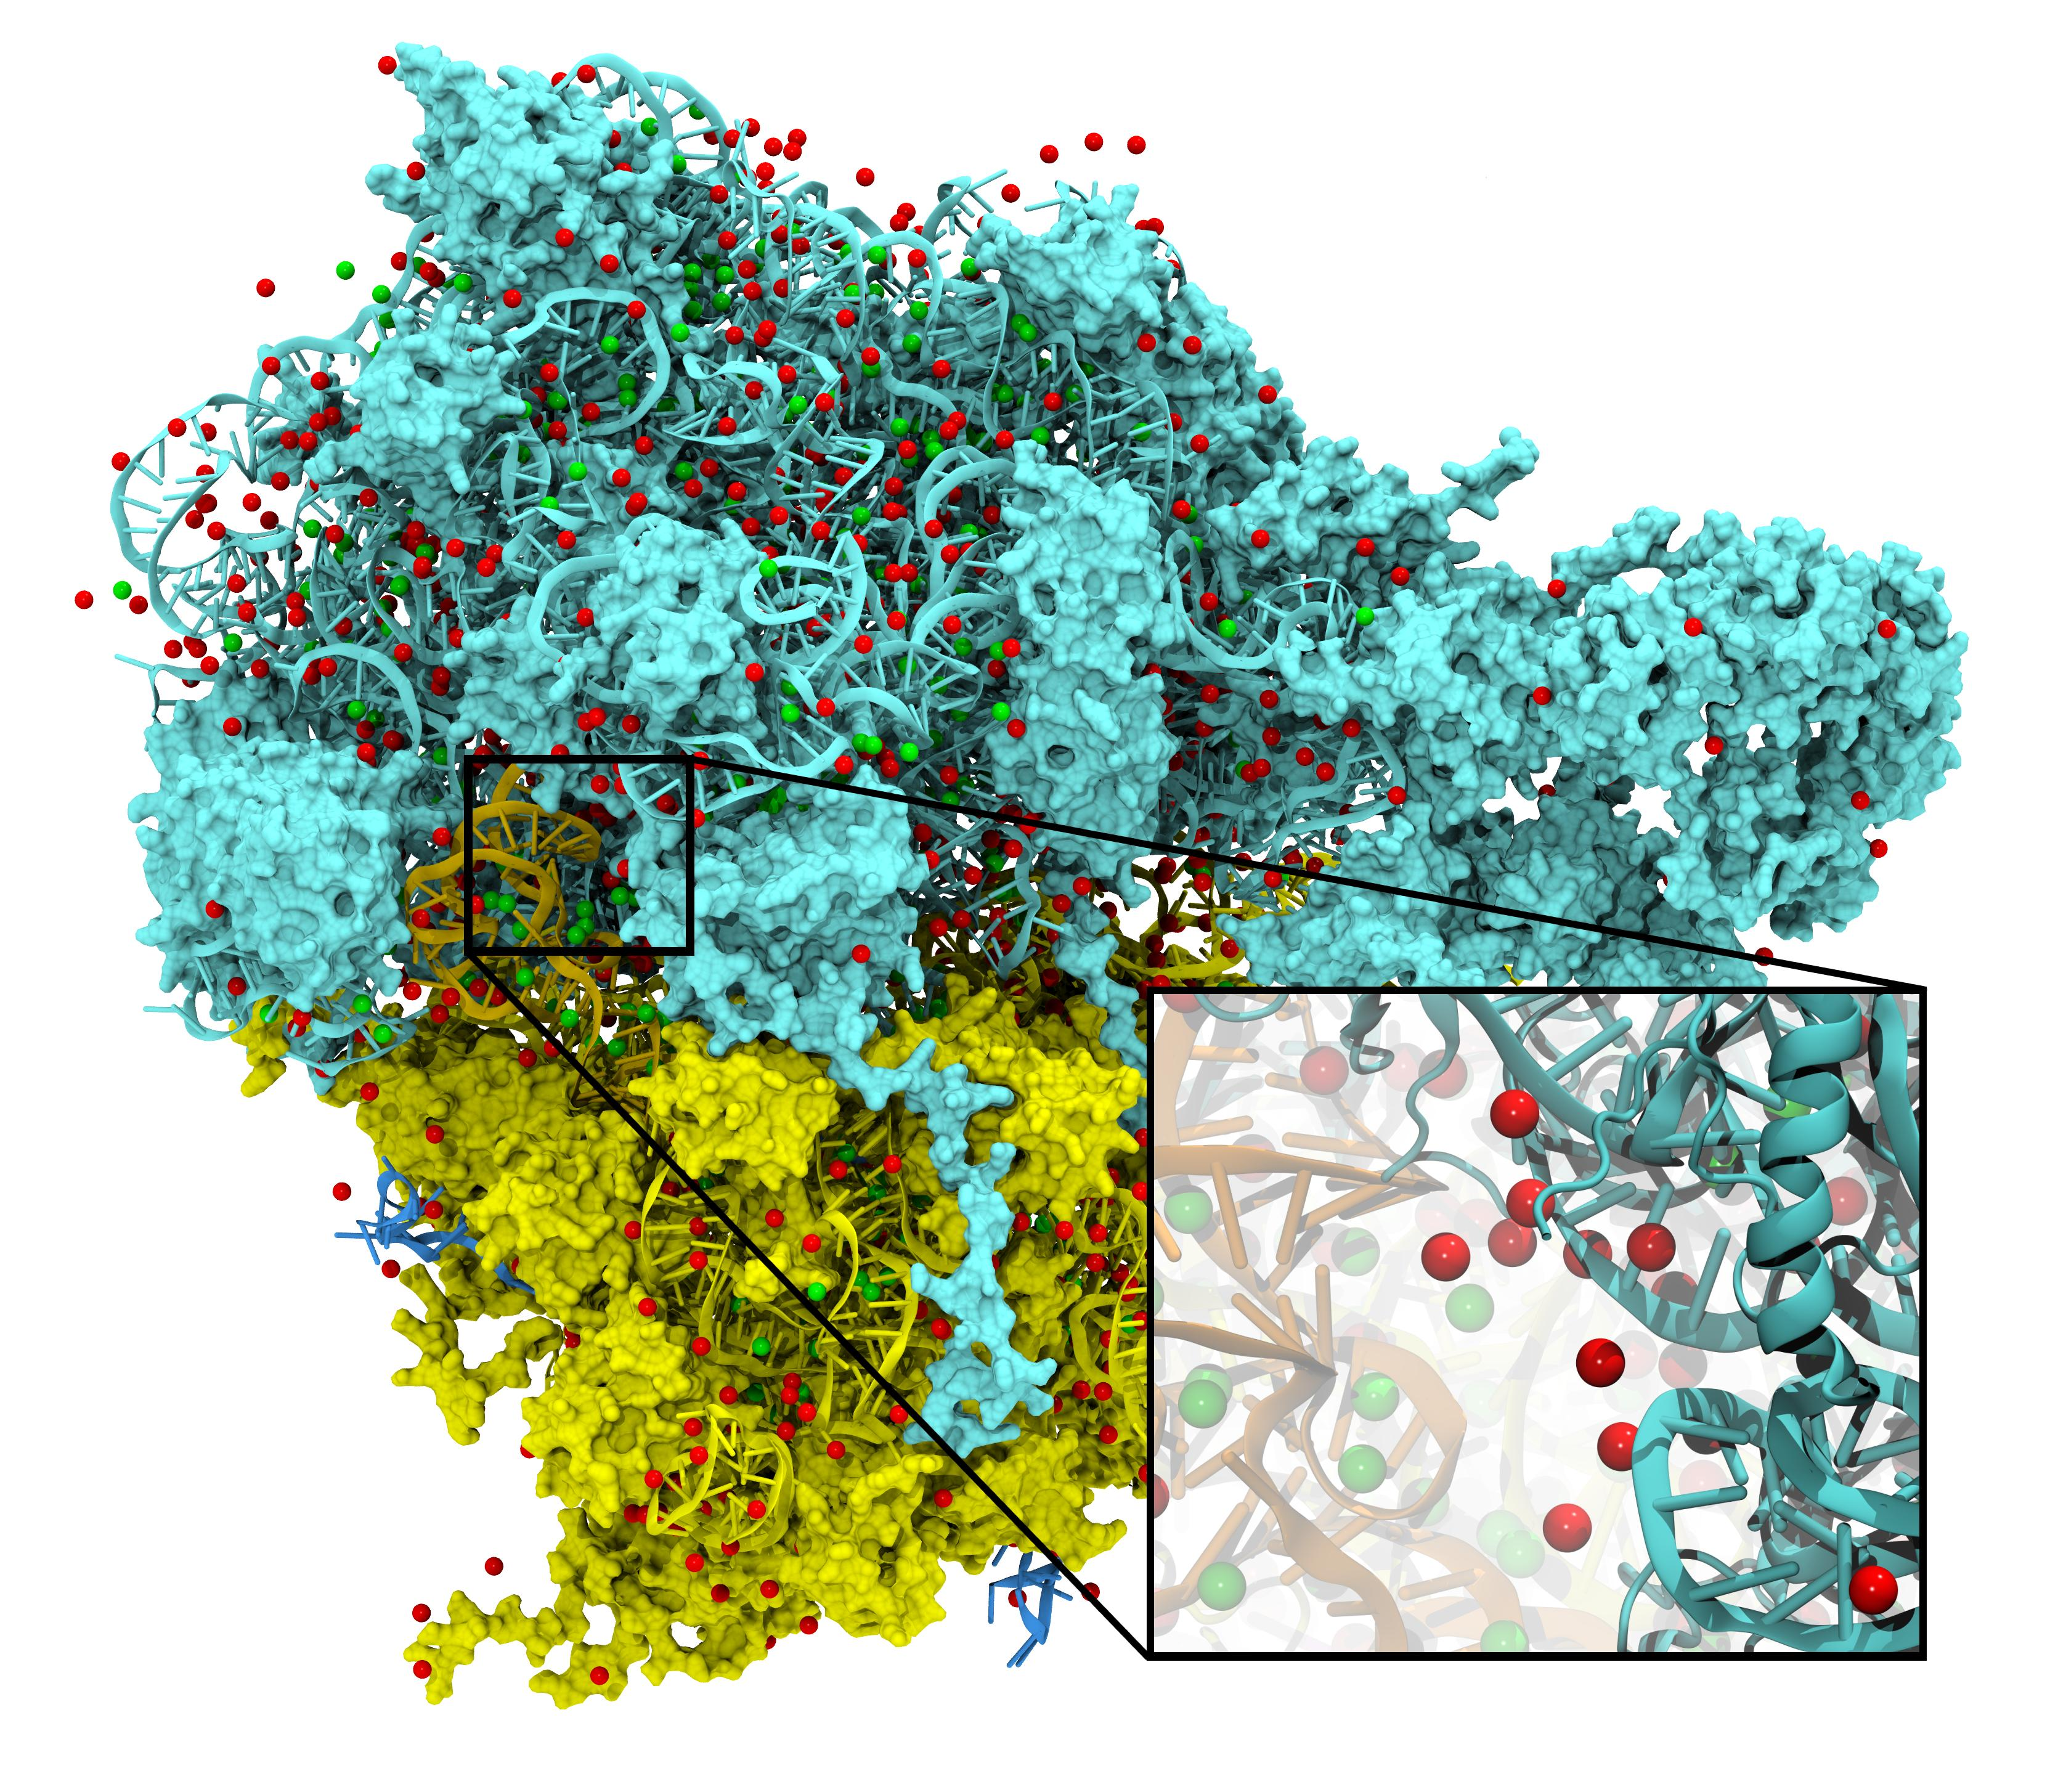
\includegraphics[width=1.0\linewidth]{complex-structure.jpg}
\end{center}
   \caption{The visualization of large bacterial ribosome structure.}
\label{fig:complex-structure}
\end{figure}

In this paper \cite{stone_immersive_2016}, researchers provides a novel solution for molecular visualization with head mounted displays(HMDs). Which achieves the performance levels required for comfortable use of HMDs while dealing with large-scale datasets and network latencies when viewing with the help of a remote server. Similar projects can also be found such as \cite{IMAX} \cite{Marsalek}. But this project combines immersive visualization techniques with high quality progressive ray tracing algorithm( implements advanced techniques such as ambient occlusion lighting, depth of field focal blur ) and supports remote rendering scenarios while achieving frame rates suitable for use in virtual environments. 

\subsection{Remote Visualization and The System Design}

Difficulties can be found in state-of-art immersive molecular visualization solutions in the rendering process. The data size and computing requirements for effective visualization will increase all the time because of the continue growing size and timescale obtained by experimental imaging (Fig. \ref{fig:complex-structure}). Regular transfer of such large amounts of data is impractical. Thus, we have to deal with large-scale datasets. When using remote visualization to eliminate the need for large file transfers, there will be a new problem: round-trip network latencies. Which would cause simulator sickness when using HMDs. Moreover, when using data streaming technique, best H.264 video encoding parameters should be found \cite{1218189}. Besides, the architecture of the system should be carefully designed.

To overcomes network latencies, they present a novel two-phase rendering approach works with the combination of omnidirectional stereoscopic progressive ray tracing and high performance rasterization \cite{hprsgpu}. They implemented that based on VMD. The system provides high-fidelity rendering previously inaccessible within immersive visualization systems. Hardware-accelerated video encoding has profoundly increased frame rates and image resolution for remote visualization. They find that the best frame rate is achieved using a single 8-GPU VCA nod. System for remotely-rendered immersive molecular visualization with HMDs designed to be a collection of components and data flow. Their system uses multithreading to maintain asynchronous execution of progressive RT and HMD display updates, with the HMD view update loop and user input handling residing in the main VMD thread.

\subsection{Rendering and Displaying Techniques}

During the rendering process, advanced rendering techniques(such as shadows, ambient occlusion lighting,depth-of-field, and high quality transparency) should also be implemented to facilitate the study of large biomolecular complexes. Besides, Speckle noise can be found in many AO lighting approximations \cite{Saadia:2018}. Uncorrelated AO sampling produces high quality converged images, but creates strong pixelated speckle noise until the image approaches convergence with a large number of accumulated samples. Again, problems has been found when accelerating with multiple GPUs. Parallel efficiency is limited by uneven work distribution in different regions of the rendered scene. During the process of omnistereo and panoramic ray tracing of biomolecular scenes, the standard planar formulations should be reimplemented with radial or spherical formulations. Including depth-of-field focal blur \cite{Kosara2004SemanticDO}, fog and depth cueing, as well as view frustum culling. In the rendered scene, The crowded molecular environment can be a dark place due to heavy shadowing with both AO and direct lighting. Which should also be fixed. When viewing with DK2 and similar HMDs, the singlet ocular lenses produce strong pincushion geometric distortion. Thus, distortion correction software should be implemented. Additionally, The 75 Hz display refresh rate of the DK2 should be achieved to provide a smoothest immersive visualization experience.

\begin{figure}[h]
\begin{center}
%\fbox{\rule{0pt}{2in} \rule{0.9\linewidth}{0pt}}
   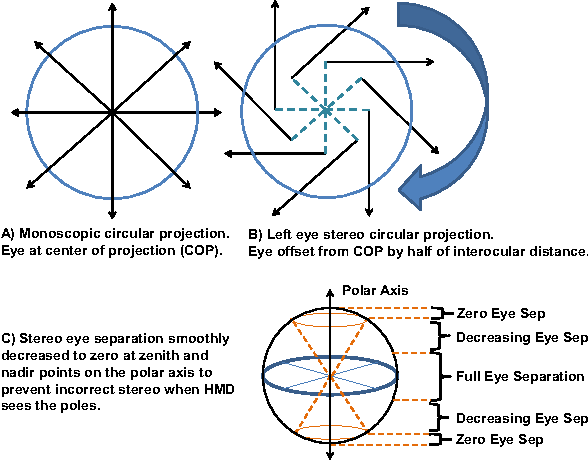
\includegraphics[width=1.0\linewidth]{projection-approach.png}
\end{center}
   \caption{The omnidirectional stereoscopic projection approach.}
\label{fig:projection-approach}
\end{figure}

To accelerate the rendering process with advanced technique such as ambient occlusion lighting, fog and depth cueing, and depth of field focal blur, they have introduced a new ray tracing algorithm used to optimize interactivity and quality. And a projection approach (Fig. \ref{fig:projection-approach}) that supports widely used spherical and cubic texture mapping operations in commodity graphics hardware. They also design and implementation a high performance progressive RT engine based on data-parallel CUDA. Direct lighting often act to obscure features of molecular structure without careful light placement while computationally inexpensive. To support advanced lighting effect for a better experience of users, they improved their progressive ray tracing algorithm. As a result, the rendering engine produces high quality images. Their RT algorithm has been accelerated using techniques like CUDA \cite{Cook:2012}, OpenCL \cite{Munshi:2011}, and ISPC \cite{Pharr2012ispcAS} , with the help of highly parallel SIMD-oriented hardware architectures. To support video streaming, they extends the TachyonLOptiX GPU-accelerated RT engine to combine video streaming technique. To get a higher performance, they update the displayed image by launching and accumulating one ormultiple images, so-called “subframes”, in each iteration. A progressive RT engine customized for immersive molecular visualization has been implemented to employ the newly designed RT. To deal with speckle noise mentioned above, they use a single random number stream to drive AO sampling for all pixelsin the same subframe. In this way, all pixels take AO lighting samples in the same direction, thereby eliminating speckle noise. The flutter effect has been eliminated. For they use a moving average to track its update rate and dynamically adjust the number of samples computed by successive subframes with the goal of maintaining a target update rate. Once the number of subframe samples has been determined, the progressive RT engine chooses a sample allocation strategy that favors image-space refinement. They found that tens of GPUs can be effectively utilized for interactive progressive rendering of complex scenes. To deal with the darkness problem, they added a point light “headlight” at the center of projection to prevent excessive darkening when viewing interiors of fully-enclosed organelles. But it produces “flat” looking shading since it is very close to the camera position. For this, they modified the AO shadow test algorithm to ignore shadows from occluding geometry beyond a maximum radius from the hit point. When displaying, their RT engine can produce a variety of omni-stereo projections including latitude-longitude,cube map and dome-master. They also developed HMD display and distortion correction software optimized both for the stock DK2 HMD and for DK2 HMDs with enhanced ocular optics. Pincushion distortion mentioned above can be neutralized by applying the inverse barrel distortion \cite{ird} prior to display. To increase the update rate during the displaying process, they use a variety of techniques to implement an HMD display loop. After that, HMD update rates can exceed 100 Hz (10 ms redraw interval) on commodity PC hardware. Where the RT engine and HMD display update loops run asynchronously in independent threads. To prevent the HMD display update loop from monopolizing the host CPUs, the display GPU, and the host PCIe bus, they make the update loop blocks on a final OpenGL buffer swap. When achieving higher performance using a host machine with slower CPUs, they developed a routine to eliminate redundancy during the upload of OpenGL textures. The worst case HMD update interval has been reduced in this way.

\subsection{Interaction}
Uncomfortable stereoscopic views can be caused when structures are too close to the camera. Which makes navigation difficult. Rendering options should be displayed in the scene to enhance the interaction process.

According to \cite{stone_immersive_2016}, to solve the navigation problem above, an optional clipping sphere feature was added to their RT engine. Objects inside the sphere (near the viewer’s eyes) are smoothly faded toward complete transparency and are ultimately clipped out entirely. To prevent clipped geometry from casting shadows, the clipping sphere also affects secondary rays. Also, They provide the user with graphical information in the form of heads-up display(HUD) and have drawn special avatar geometry that represents the user’s wand.

\section{Visualization of Atomistic Simulations}
\subsection{Overview}
Reda et al. \cite{reda_visualizing_2013} present an application for interactive visualization and exploration of large-scale atomistic simulations in ultra-resolution immersive environments on the CAVE2 \cite{febretti2013cave2} (Fig. \ref{img:atomistic1}). The CAVE2 is a cylindrical immersive environment consisting of 72 micro-polarized, passive stereo LCD panels that are arrange on the circumference of the cylinder, providing a 320-degrees panoramic view at a total stereoscopic resolution of 74 Megapixels. Molecular Dynamics (MD) is a principle methodology in the study of nanoscale systems in applications of alternative fuel, battery design or energy storage. MD simulations usually consist of tens to hundreds of million atoms in complex structures, leading to many challenges in visualization and analysis. Computational chemists, physicists, and materials scientists evaluated the system. Even though there are a lot of molecular visualization techniques, atomistic simulations remain difficult. Real-time rendering of molecular surfaces is also prohibitively expensive. Here they are using a hybrid representation, which combines a ball-and-stick glyph (to show the molecule itself) with volumetric surfaces to show the uncertainty in molecular boundaries at the nanoscale. For evaluation, four different data sets with up to 15 million atoms were used. The goals of the project were to show the scalability and the desire to highlight emergent high-level features in the molecular structure. Furthermore, they wanted to enable scientists to explore different boundary interpretations of atoms or molecules.

\setlength{\parindent}{1pc}This approach has some similarities to the project of chapter 4 as molecules are visualized, but it is difference in the sense that the other project focuses on ray-tracing with the setup of HMDs. Furthermore the project of chapter 3 has some similarities as it visualizing volumetric data as well, but is using isosurface rendering rather than volume rendering.

\subsection{Rendering}
\begin{figure}
	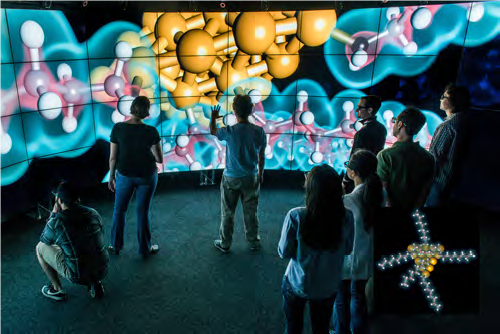
\includegraphics{atomistic_4.png}
	\caption{Visulization of electronic structures}
	\label{img:atomistic1}
\end{figure}
\begin{figure}
	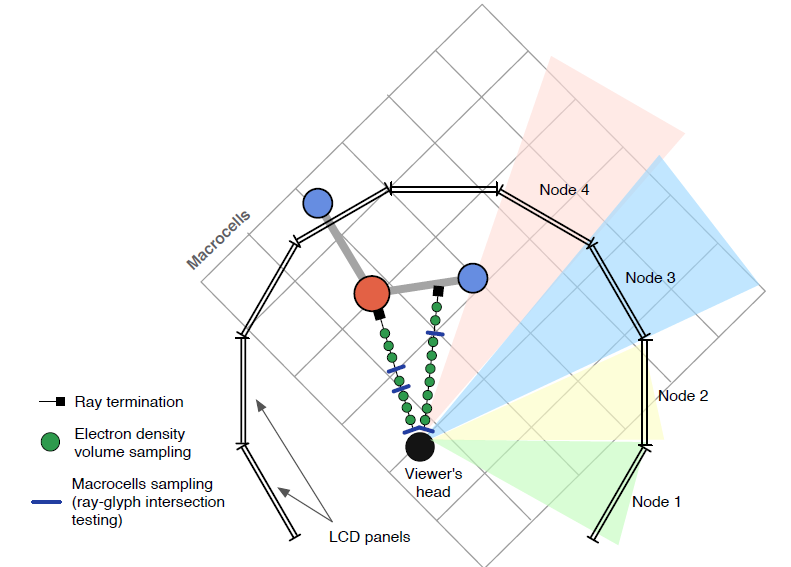
\includegraphics{atomistic_6.png}
	\caption{Illustration of the immersive, distributed ray-casting process}
	\label{img:atomistic2}
\end{figure}

The main techniques they used are ray-casting and volume rendering. Ray-casting is a rendering technique that is done pixel-wise. For every pixel a ray from the viewer is evaluated for intersecting objects. Direct volume rendering is a technique to show a volume data set. Therefore, every sample value is mapped to an opacity and a color via a transfer function. Here, they employed direct volume rendering to render the approximate electron densities. This enables a variety of visual representations by varying the transfer function, which then allows for a flexible interpretation of the molecular boundaries. The volume rendering was very useful for visual classification. For example in one data set (a nanoscale simulation of an amorphous glass (SiO2) fracture), scientists were able to segment the amorphous aluminum shell from the aluminum core. For computational chemists the hybrid volume + glyph technique proved to be more flexible than classical isosurface techniques as they need to see molecule and the electronic structure. The volume rendering also seemed to naturally decrease the visual clutter by creating a 'fog' effect, which reduced the interference with the distant atoms.

\setlength{\parindent}{1pc}As a data structure to represent the ball-and-stick glyphs, a uniform 'Macrocells' 3D grid stored in the GPU is employed. Each voxel in the grid stores information about all of the atoms and bonds, which are within the cell. Therefore only pointers to a separate array are stored, because overlapping glyphs are represented in multiple cells. The ray-casting algorithm \cite{Amanatides87afast} traverses each voxel at a discrete level (Fig. \ref{img:atomistic2}). Because the list of glyphs in a cell is not depth ordered, the algorithm has to test every primitive (sphere or cylinder) against the ray. After a hit is found, the surface of the closest glyph is Phong shaded. Afterward, the charge density volume is sampled within the current cell and the color is accumulated according to the transfer function. Empty Macrocells are skipped and the ray stops when the accumulated volume opacity saturates the pixel- For the electron charge densities, they either used a precomputed electron density grid or a real-time density computation on the GPU. Using precomputed values the algorithm was 2-3 times faster, which was no surprise as the computation is quite expensive. For real time computation of the electron densities they used an approximation with Gaussian distribution based on Van der Waals radii of the atoms or averaged from density functional theory (DFT) computations.

\setlength{\parindent}{1pc}To speed up rendering, an in-core solution was applied making sure that at least one time step of the simulation is loaded into the GPU memory of all rendering nodes. In the CAVE2 \cite{febretti2013cave2} system they employed a 36-node-cluster to render the immersive visualization on 72 LCD panels in parallel. The Ray-cast is done users head to each panel (Fig. \ref{img:atomistic2}). To achieve stereoscopic rendering, rendering and interleaving two images separated by the average inter-pupillary distance is applied. To support correct viewing for multiple individuals, they normalized the head orientation when tracking, so that the eyes are always parallel to the screens surface. That might lead to small distortions between the tiles but it described as a good compromise. 

\setlength{\parindent}{1pc}They were able to achieve real-time interactive rendering when using precomputed electron densities for all of their four tested data sets. Up to 5 million atoms the algorithm scaled solidly with an average frame rate of 15 FPS. With 15 million atoms the frame rate halves but they still achieved interactive rendering at 7 FPS. When the electron densities were computed in real-time, reasonable interactive speeds were achieved for 3 out of 4 data sets. So there are still remaining challenges for optimization of real-time computed electronic densities for atomistic simulations.

\subsection{Interaction}
The CAVE2 \cite{febretti2013cave2} provides 3D navigation using a 6 degrees-of-freedom joystick coupled with head-tracking. The user can fly through the simulation by using a button and by moving/rotating the joystick in the desired direction. Wireless head-tracking also enables the user to explore the visualization by physically walking in the space, causing the view to be rendered from his/her perspective. The head-tracking provides a user-centered perspective. The user can also adjust the transfer function or the color of the electron density ranges by the wireless 'wand' or via separate interface on a tablet or laptop. The modification updates the visualization in real-time. Opacity of the volume and quality of the rendering can also be changed interactively.

\subsection{Conclusion}
As conventional molecular surfaces are not appropriate for many nanomaterials because they do not show the uncertainty in boundaries. The author of the paper showed a hybrid visual metaphor for the visualization complex nanostructured material via volume rendering of approximated electron densities, which proposed advantages. Future work still needs to be done to improve the run-time especially with very large data sets.

\section{Conclusion}

{\small
\bibliographystyle{unsrt}
\bibliography{reviewbib}
}

\end{document}
